\documentclass[12pt,a4paper]{article}
\usepackage[utf8]{inputenc}
\usepackage[T1]{fontenc}
\usepackage{lmodern}
\usepackage{microtype}
\usepackage{graphicx}
\usepackage{tikz}
\usepackage{pgfplots}
\usepackage{booktabs}
\usepackage{array}
\usepackage{multirow}
\usepackage{listings}
\usepackage{xcolor}
\usepackage{hyperref}
\usepackage{fancyhdr}
\usepackage{amsmath}
\usepackage{amssymb}
\usepackage{algorithm2e}
\usepackage{float}
\usepackage{caption}
\usepackage{subcaption}
\usepackage{upquote} 

% TikZ libraries
\usetikzlibrary{shapes.geometric, arrows, positioning, calc, shadows, patterns, decorations.pathreplacing}
\pgfplotsset{compat=1.17}

% Fix headheight warning
\setlength{\headheight}{14.5pt}
\setlength{\headsep}{0.2in}
\setlength{\topmargin}{-0.25in}
\setlength{\textheight}{9.0in}
\setlength{\textwidth}{6.5in}
\setlength{\oddsidemargin}{0in}
\setlength{\evensidemargin}{0in}

% If you're using the geometry package, use this instead:
% \usepackage[headheight=14.5pt,headsep=0.2in,top=1in,bottom=1in,left=1in,right=1in]{geometry}

% \definecolor{vc_pink}{RGB}{255,0,220}
% \definecolor{vc_cyan}{RGB}{0,170,255}
% \definecolor{fn_purple}{RGB}{130,0,130}
% \definecolor{fn_orange}{RGB}{255,140,0}
% \definecolor{vc_green}{RGB}{0,100,70}
% \definecolor{vc_bg}{RGB}{250,250,240}

% \lstdefinestyle{customc}{
%   % language=JavaScript,
%   backgroundcolor=\color{vc_bg},
%   commentstyle=\color{vc_cyan},
%   keywordstyle=\color{vc_pink},
%   numberstyle=\tiny\color{fn_purple},
%   stringstyle=\color{vc_green},
%   basicstyle=\footnotesize\ttfamily,
%   breaklines=true,
%   breakatwhitespace=true,
%   tabsize=4,
%   numbers=left,
%   numbersep=10pt,
%   showstringspaces=false,
% }

% \lstset{style=customc}

% \lstdefinelanguage{JavaScript}{
%   keywords={typeof, new, true, false, catch, function, return, null, catch, switch, var, if, in, while, do, else, case, break},
%   keywordstyle=\color{blue}\bfseries,
%   ndkeywords={class, export, boolean, throw, implements, import, this},
%   ndkeywordstyle=\color{darkgray}\bfseries,
%   identifierstyle=\color{black},
%   sensitive=false,
%   comment=[l]{//},
%   morecomment=[s]{/*}{*/},
%   commentstyle=\color{purple}\ttfamily,
%   stringstyle=\color{red}\ttfamily,
%   morestring=[b]',
%   morestring=[b]"
% }

% \lstset{
%    language=JavaScript,
%    backgroundcolor=\color{lightgray},
%    extendedchars=true,
%    basicstyle=\footnotesize\ttfamily,
%    showstringspaces=false,
%    showspaces=false,
%    numbers=left,
%    numberstyle=\footnotesize,
%    numbersep=9pt,
%    tabsize=2,
%    breaklines=true,
%    showtabs=false,
%    captionpos=b
% }

% Add these color definitions to your preamble
\definecolor{vc_pink}{RGB}{255,0,220}
\definecolor{vc_cyan}{RGB}{0,170,255}
\definecolor{fn_purple}{RGB}{130,0,130}
\definecolor{fn_orange}{RGB}{255,140,0}
\definecolor{vc_green}{RGB}{0,100,70}
\definecolor{vc_bg}{RGB}{250,250,240}

% Base style
\lstdefinestyle{base_style}{
    backgroundcolor=\color{vc_bg},
    basicstyle=\footnotesize\ttfamily,
    breaklines=true,
    breakatwhitespace=true,
    tabsize=4,
    numbers=left,
    numbersep=10pt,
    numberstyle=\tiny\color{fn_purple},
    showstringspaces=false,
    captionpos=b,
    frame=single,
    rulecolor=\color{lightgray},
    xleftmargin=15pt,
    framexleftmargin=15pt
}

% JavaScript style
\lstdefinestyle{javascript}{
    style=base_style,
    language=JavaScript,
    keywordstyle=\color{vc_pink}\bfseries,
    commentstyle=\color{vc_cyan}\itshape,
    stringstyle=\color{vc_green},
    morekeywords={let, const, async, await, export, import, from, as, default, class, extends, super, constructor, static, get, set, of, in, instanceof, typeof, yield, interface, type, implements},
    morecomment=[l]{//},
    morecomment=[s]{/*}{*/},
    morestring=[b]',
    morestring=[b]",
    morestring=[b]`,
    moredelim=*[s][\color{fn_orange}]{/*@}{\*/},
    moredelim=*[s][\color{fn_orange}]{/**}{\*/},
    moredelim=*[s][\color{fn_orange}]{//!}{},
    moredelim=*[s][\color{fn_orange}]{//?}{},
    moredelim=*[s][\color{fn_orange}]{//.}{},
    moredelim=*[s][\color{fn_orange}]{//:}{},
    moredelim=*[s][\color{fn_orange}]{//|}{},
    moredelim=*[s][\color{fn_orange}]{//!<}{},
    moredelim=*[s][\color{fn_orange}]{//!>}{}
}

% Dart style
% \lstdefinestyle{Dart}{
%     style=base_style,
%     language=Dart, % Using Java as base since Dart is not natively supported
%     keywordstyle=\color{vc_pink}\bfseries,
%     commentstyle=\color{vc_cyan}\itshape,
%     stringstyle=\color{vc_green},
%     morekeywords={
%         % Dart specific keywords
%         abstract, as, assert, async, await, break, case, catch, class, const,
%         continue, covariant, default, deferred, do, dynamic, else, enum, export,
%         extension, external, extends, factory, false, final, finally, for, Function,
%         get, hide, if, implements, import, in, interface, is, library, mixin, new,
%         null, on, operator, part, rethrow, return, set, show, static, super, switch,
%         sync, this, throw, true, try, typedef, var, void, while, with, yield, yield*
%     },
%     morecomment=[l]{//},
%     morecomment=[s]{/*}{*/},
%     morestring=[b]',
%     morestring=[b]",
%     morestring=[b]''',
%     morestring=[b]""",
%     moredelim=*[s][\color{fn_orange}]{///}{},
%     moredelim=*[s][\color{fn_orange}]{//!}{},
%     moredelim=*[s][\color{fn_orange}]{//?}{},
%     moredelim=*[s][\color{fn_orange}]{//.}{},
%     moredelim=*[s][\color{fn_orange}]{//:}{},
%     moredelim=*[s][\color{fn_orange}]{//|}{}
% }

\lstdefinestyle{dart}{
    style=base_style,
    language=Dart,
    keywordstyle=\color{vc_pink}\bfseries,
    commentstyle=\color{vc_cyan}\itshape,
    stringstyle=\color{vc_green},
    numberstyle=\tiny\color{fn_purple},
    keywordstyle=[2]\color{fn_orange},
    keywordstyle=[3]\color{fn_orange}\itshape,
    moredelim=[s][\color{vc_pink}\bfseries]{\?}{:},
    moredelim=[s][\color{vc_pink}\bfseries]{\?\?}{},
    moredelim=[s][\color{vc_pink}\bfseries]{\?\.}{}
}

% Set default style
\lstset{style=base_style}

% Define JavaScript language
\lstdefinelanguage{JavaScript}{
    keywords={typeof, new, true, false, catch, function, return, null, catch, switch, var, if, in, while, do, else, case, break, let, const, async, await, export, import, from, as, default, class, extends, super, constructor, static, get, set, of, in, instanceof, typeof, yield, interface, type, implements},
    ndkeywords={class, export, boolean, throw, implements, import, this, string, number, boolean, void, any, never, unknown, object, symbol, bigint, undefined, null, true, false, enum, type, interface, namespace, module, declare, as, is, keyof, infer, extends, readonly, required, Partial, Pick, Omit, ReturnType, Parameters, ConstructorParameters, ThisType, NonNullable, Uppercase, Lowercase, Capitalize, Uncapitalize},
    sensitive=true,
    comment=[l]{//},
    morecomment=[s]{/*}{*/},
    morestring=[b]',
    morestring=[b]",
    morestring=[b]`,
    morestring=[s]{"""*}{"""},
    morestring=[s]{'''*}{'''},
    morecomment=[l][\color{vc_cyan}]{///},
    morecomment=[l][\color{vc_cyan}]{//!},
    morecomment=[l][\color{vc_cyan}]{//?},
    morecomment=[l][\color{vc_cyan}]{//.},
    morecomment=[l][\color{vc_cyan}]{//:},
    morecomment=[l][\color{vc_cyan}]{//|},
    morecomment=[s][\color{vc_cyan}]{/**}{*/},
    morecomment=[s][\color{vc_cyan}]{/*!}{*/},
    morecomment=[s][\color{vc_cyan}]{/*?}{*/},
    morecomment=[s][\color{vc_cyan}]{/*.}{*/},
    morecomment=[s][\color{vc_cyan}]{/*:}{*/},
    morecomment=[s][\color{vc_cyan}]{/*|}{*/}
}

% Define Dart language
\lstdefinelanguage{Dart}{
    % Basic keywords
    keywords={
        abstract, as, assert, async, await, break, case, catch, class, const,
        continue, covariant, default, deferred, do, dynamic, else, enum, export,
        extension, external, extends, factory, false, final, finally, for, Function,
        get, hide, if, implements, import, in, interface, is, library, mixin, new,
        null, on, operator, part, rethrow, return, set, show, static, super, switch,
        sync, this, throw, true, try, typedef, var, void, while, with, yield, yield*,
        required, late
    },
    % Type system and built-ins
    morekeywords=[2]{int, double, num, bool, String, List, Set, Map, Runes, Symbol, 
        Object, Null, Never, dynamic, void, Future, Stream, Iterable, DateTime, 
        Duration, BigInt, RegExp, Type, Error, Exception, StackTrace, Uri
    },
    % Annotations
    morekeywords=[3]{@override, @deprecated, @required, @protected, 
        @visibleForTesting, @mustCallSuper, @sealed, @immutable, @optionalTypeArgs
    },
    sensitive=true,
    % Comments
    comment=[l]{//},
    morecomment=[s]{/*}{*/},
    % Documentation comments
    morecomment=[l][\color{vc_cyan}]{///},
    morecomment=[l][\color{vc_cyan}]{//!},
    morecomment=[s][\color{vc_cyan}]{/**}{*/},
    % Strings
    morestring=[b]',
    morestring=[b]",
    morestring=[b]''',
    morestring=[b]""",
    % String interpolation
    % moredelim=[s][\color{vc_green}]{${}{\}},
    % moredelim=[s][\color{vc_green}]{${\{}{\}}},
    % Raw strings
    morestring=[s][\color{vc_green}]{r'}{'},
    morestring=[s][\color{vc_green}]{r"}{"},
    morestring=[s][\color{vc_green}]{r'''}{'''},
    morestring=[s][\color{vc_green}]{r"""}{"""},
    % Numbers
    moredelim=[s][\color{fn_purple}]{0x}{[0-9a-fA-F]+},
    moredelim=[s][\color{fn_purple}]{0b}{[01]+},
    moredelim=[s][\color{fn_purple}]{0o}{[0-7]+},
    moredelim=[s][\color{fn_purple}]{[0-9]}{[0-9.eE+\-]+}
}
% Define Dart language
% \lstdefinelanguage{Dart}{
%     % Basic keywords
%     keywords={
%         abstract, as, assert, async, await, break, case, catch, class, const,
%         continue, covariant, default, deferred, do, dynamic, else, enum, export,
%         extension, external, extends, factory, false, final, finally, for, Function,
%         get, hide, if, implements, import, in, interface, is, library, mixin, new,
%         null, on, operator, part, rethrow, return, set, show, static, super, switch,
%         sync, this, throw, true, try, typedef, var, void, while, with, yield, yield*,
%         required, late, required, required, required, required, required, required,
%         required, required, required, required, required, required, required
%     },
%     % Type system and built-ins
%     ndkeywords={
%         int, double, num, bool, String, List, Set, Map, Runes, Symbol, Object, Null,
%         Never, dynamic, void, Future, Stream, Iterable, DateTime, Duration, BigInt,
%         RegExp, Type, Error, Exception, StackTrace, Uri, bool, double, int, num, String,
%         Comparable, Pattern, Iterator, MapEntry, Match, Null, Object, Pattern, RegExp,
%         Set, Sink, StackTrace, Stream, String, StringBuffer, StringSink, Symbol, Type,
%         Uri, bool, double, int, num, String, Map, List, Set, Runes, Symbol, Object, Null,
%         Never, dynamic, void, Future, Stream, Iterable, DateTime, Duration, BigInt,
%         RegExp, Type, Error, Exception, StackTrace, Uri, bool, double, int, num, String,
%         Comparable, Pattern, Iterator, MapEntry, Match, Null, Object, Pattern, RegExp,
%         Set, Sink, StackTrace, Stream, String, StringBuffer, StringSink, Symbol, Type, Uri
%     },
%     sensitive=true,
%     % Comments
%     comment=[l]{//},
%     morecomment=[s]{/*}{*/},
%     % Strings
%     morestring=[b]',
%     morestring=[b]",
%     morestring=[b]''',
%     morestring=[b]""",
%     % Documentation comments
%     morecomment=[l][\color{vc_cyan}]{///},
%     morecomment=[l][\color{vc_cyan}]{//!},
%     morecomment=[s][\color{vc_cyan}]{/**}{*/},
%     morecomment=[s][\color{vc_cyan}]{/*!}{*/},
%     % Annotations
%     morekeywords=[2]{@override, @deprecated, @required, @protected, @visibleForTesting, @mustCallSuper,
%         @sealed, @immutable, @protected, @optionalTypeArgs, @protected, @protected, @protected,
%         @protected, @protected, @protected, @protected, @protected, @protected, @protected,
%         @protected, @protected, @protected, @protected, @protected, @protected, @protected,
%         @protected, @protected, @protected, @protected, @protected, @protected, @protected,
%         @protected, @protected, @protected, @protected, @protected, @protected, @protected
%     },
%     keywordstyle=[2]\color{fn_orange},
%     % Built-in types
%     morekeywords=[3]{int, double, num, bool, String, List, Set, Map, Runes, Symbol, Object, Null,
%         Never, dynamic, void, Future, Stream, Iterable, DateTime, Duration, BigInt, RegExp
%     },
%     keywordstyle=[3]\color{vc_pink},
%     % String interpolation
%     % moredelim=[s][\color{vc_green}]{${}{\}},
%     % moredelim=[s][\color{vc_green}]{${\{}{\}}},
%     % Raw strings
%     morestring=[s][\color{vc_green}]{r'}{'},
%     morestring=[s][\color{vc_green}]{r"}{"},
%     % Multiline strings
%     morestring=[s][\color{vc_green}]{r'''}{'''},
%     morestring=[s][\color{vc_green}]{r"""}{"""},
%     % Numbers
%     moredelim=[s][\color{fn_purple}]{0x}{[0-9a-fA-F]+},
%     moredelim=[s][\color{fn_purple}]{0b}{[01]+},
%     moredelim=[s][\color{fn_purple}]{0o}{[0-7]+},
%     moredelim=[s][\color{fn_purple}]{[0-9]}{[0-9.eE+\-]+},
%     % Operators
%     moredelim=[s][\color{vc_pink}\bfseries]{?}{:},
%     moredelim=[s][\color{vc_pink}\bfseries]{??}{},
%     moredelim=[s][\color{vc_pink}\bfseries]{?.}{},
%     moredelim=[s][\color{vc_pink}\bfseries]{!}{},
%     moredelim=[s][\color{vc_pink}\bfseries]{?}{},
%     moredelim=[s][\color{vc_pink}\bfseries]{..}{},
%     moredelim=[s][\color{vc_pink}\bfseries]{...}{},
%     moredelim=[s][\color{vc_pink}\bfseries]{~}{},
%     moredelim=[s][\color{vc_pink}\bfseries]{*}{},
%     moredelim=[s][\color{vc_pink}\bfseries]{/}{},
%     moredelim=[s][\color{vc_pink}\bfseries]{\%}{},
%     moredelim=[s][\color{vc_pink}\bfseries]{+}{},
%     moredelim=[s][\color{vc_pink}\bfseries]{-}{},
%     moredelim=[s][\color{vc_pink}\bfseries]{<<}{},
%     moredelim=[s][\color{vc_pink}\bfseries]{>>}{},
%     moredelim=[s][\color{vc_pink}\bfseries]{>>>}{},
%     moredelim=[s][\color{vc_pink}\bfseries]{<}{=},
%     moredelim=[s][\color{vc_pink}\bfseries]{>}{=},
%     moredelim=[s][\color{vc_pink}\bfseries]{==}{},
%     moredelim=[s][\color{vc_pink}\bfseries]{!=}{},
%     moredelim=[s][\color{vc_pink}\bfseries]{===}{},
%     moredelim=[s][\color{vc_pink}\bfseries]{\&}{},
%     moredelim=[s][\color{vc_pink}\bfseries]{\^{}}{},
%     moredelim=[s][\color{vc_pink}\bfseries]{\|}{},
%     moredelim=[s][\color{vc_pink}\bfseries]{\&\&}{},
%     moredelim=[s][\color{vc_pink}\bfseries]{\|\|}{},
%     moredelim=[s][\color{vc_pink}\bfseries]{??}{=},
%     moredelim=[s][\color{vc_pink}\bfseries]{??=}{},
%     moredelim=[s][\color{vc_pink}\bfseries]{..}{=},
%     moredelim=[s][\color{vc_pink}\bfseries]{~/}{},
%     moredelim=[s][\color{vc_pink}\bfseries]{~/}{=},
%     moredelim=[s][\color{vc_pink}\bfseries]{*}{=},
%     moredelim=[s][\color{vc_pink}\bfseries]{/}{=},
%     moredelim=[s][\color{vc_pink}\bfseries]{\%}{=},
%     moredelim=[s][\color{vc_pink}\bfseries]{+}{=},
%     moredelim=[s][\color{vc_pink}\bfseries]{-}{=},
%     moredelim=[s][\color{vc_pink}\bfseries]{<<}{=},
%     moredelim=[s][\color{vc_pink}\bfseries]{>>}{=},
%     moredelim=[s][\color{vc_pink}\bfseries]{>>>}{=},
%     moredelim=[s][\color{vc_pink}\bfseries]{\&}{=},
%     moredelim=[s][\color{vc_pink}\bfseries]{\^{}}{=},
%     moredelim=[s][\color{vc_pink}\bfseries]{\|}{=},
%     moredelim=[s][\color{vc_pink}\bfseries]{??}{=},
%     moredelim=[s][\color{vc_pink}\bfseries]{??=}{=},
%     moredelim=[s][\color{vc_pink}\bfseries]{..}{=},
%     moredelim=[s][\color{vc_pink}\bfseries]{??=}{},
%     moredelim=[s][\color{vc_pink}\bfseries]{..}{},
%     moredelim=[s][\color{vc_pink}\bfseries]{...}{},
%     moredelim=[s][\color{vc_pink}\bfseries]{...?}{},
%     moredelim=[s][\color{vc_pink}\bfseries]{?}{.},
%     moredelim=[s][\color{vc_pink}\bfseries]{?}{[]},
%     moredelim=[s][\color{vc_pink}\bfseries]{?}{()},
%     moredelim=[s][\color{vc_pink}\bfseries]{?}{.}{},
%     moredelim=[s][\color{vc_pink}\bfseries]{?}{[]}{},
%     moredelim=[s][\color{vc_pink}\bfseries]{?}{()}{},
%     moredelim=[s][\color{vc_pink}\bfseries]{?}{.}{.}{},
%     moredelim=[s][\color{vc_pink}\bfseries]{?}{[]}{.}{},
%     moredelim=[s][\color{vc_pink}\bfseries]{?}{()}{.}{},
%     moredelim=[s][\color{vc_pink}\bfseries]{?}{.}{.}{.}{},
%     moredelim=[s][\color{vc_pink}\bfseries]{?}{[]}{.}{.}{},
%     moredelim=[s][\color{vc_pink}\bfseries]{?}{()}{.}{.}{}
% }

% Define Dart language
\lstdefinelanguage{Dart}{
    basicstyle=\ttfamily\small,
    keywords={abstract, as, assert, async, await, break, case, catch, class, const,
        continue, covariant, default, deferred, do, dynamic, else, enum, export,
        extension, external, extends, factory, false, final, finally, for, Function,
        get, hide, if, implements, import, in, interface, is, library, mixin, new,
        null, on, operator, part, rethrow, return, set, show, static, super, switch,
        sync, this, throw, true, try, typedef, var, void, while, with, yield, yield*,
        required, late},
    morecomment=[l]{//},
    morecomment=[s]{/*}{*/},
    morestring=[b]',
    morestring=[b]",
    morestring=[b]''',
    morestring=[b]""",
    sensitive=true
}

\lstdefinestyle{dartstyle}{
    language=Dart,
    backgroundcolor=\color{vc_bg},
    basicstyle=\ttfamily\small,
    keywordstyle=\color{vc_pink}\bfseries,
    commentstyle=\color{vc_cyan}\itshape,
    stringstyle=\color{vc_green},
    numberstyle=\tiny\color{fn_purple},
    breaklines=true,
    breakatwhitespace=true,
    tabsize=2,
    numbers=left,
    numbersep=5pt,
    showstringspaces=false,
    captionpos=b,
    frame=single,
    rulecolor=\color{lightgray},
    xleftmargin=15pt,
    framexleftmargin=15pt
}

% Usage examples:
% \begin{lstlisting}[style=javascript]
% // Your JavaScript code here
% \end{lstlisting}
% 
% \begin{lstlisting}[style=dart]
% // Your Dart code here
% \end{lstlisting}

% Code listing settings
% \lstset{
%     basicstyle=\ttfamily\footnotesize,
%     breaklines=true,
%     keywordstyle=\color{blue}\bfseries,
%     commentstyle=\color{green!60!black},
%     stringstyle=\color{red},
%     showstringspaces=false,
%     numbers=left,
%     numberstyle=\tiny\color{gray},
%     frame=single,
%     backgroundcolor=\color{gray!10},
%     captionpos=b,
%     tabsize=2
% }

% Hyperlink settings
\hypersetup{
    colorlinks=true,
    linkcolor=blue,
    urlcolor=blue,
    citecolor=blue
}

% Page layout
\pagestyle{fancy}
\fancyhf{}
\fancyhead[L]{Socket Programming Lab 1}
\fancyhead[R]{Cross-Computer File Transfer}
\fancyfoot[C]{\thepage}

% Title information
\title{
    \textbf{Socket Programming Lab 1} \\
    \large Cross-Computer File Transfer \\
    \vspace{0.5cm}
    \includegraphics[width=0.3\textwidth]{network_diagram.png}
}
\author{
    Student A: LS2025001 \\
    Student B: LS2024002 \\
    \vspace{0.3cm}
    Department of Computer Science \\
    \vspace{0.3cm}
    \today
}
\date{}

\begin{document}

% \maketitle
\input{portada}
\tableofcontents
\newpage

%===============================================================================
\section{Introduction}
%===============================================================================

This laboratory experiment focuses on implementing cross-computer file transfer using socket programming. The objective is to understand the fundamental principles of network communication, master bidirectional client-server architecture, and develop practical skills in configuring network environments for real-world applications.

\subsection{Learning Objectives}
\begin{itemize}
    \item Understand socket programming fundamentals and TCP/IP communication
    \item Master bidirectional client-server communication patterns
    \item Learn to configure network environments for actual communication
    \item Develop teamwork and problem-solving skills in network programming
    \item Implement file integrity verification and error handling
    \item Create user-friendly interfaces for file transfer operations
\end{itemize}

\subsection{Technical Requirements}
\begin{itemize}
    \item \textbf{Hardware}: Two computers on the same local area network
    \item \textbf{Software}: Python 3.7+, Node.js 16+, Flutter 3.10+
    \item \textbf{Network}: Same subnet with firewall configuration
    \item \textbf{Protocols}: TCP sockets for reliable data transmission
\end{itemize}

%===============================================================================
\section{Theoretical Background}
%===============================================================================

\subsection{Socket Programming Fundamentals}

Sockets provide a programming interface for network communication between processes. They act as endpoints for sending and receiving data across a network. The socket API abstracts the complexities of network protocols, allowing developers to focus on application logic.

\subsubsection{TCP vs UDP}
\begin{table}[H]
\centering
\begin{tabular}{|l|p{5cm}|p{5cm}|}
\hline
\textbf{Characteristic} & \textbf{TCP (Transmission Control Protocol)} & \textbf{UDP (User Datagram Protocol)} \\
\hline
Connection & Connection-oriented & Connectionless \\
\hline
Reliability & Reliable, ordered delivery & Unreliable, no guarantee \\
\hline
Speed & Slower due to overhead & Faster, minimal overhead \\
\hline
Use Case & File transfer, web browsing & Streaming, gaming \\
\hline
\end{tabular}
\caption{Comparison of TCP and UDP protocols}
\end{table}

For this laboratory, we use TCP sockets to ensure reliable file transfer with guaranteed delivery and data integrity.

\subsubsection{Socket API Functions}
\begin{itemize}
    \item \texttt{socket()}: Create a new socket
    \item \texttt{bind()}: Associate socket with network address
    \item \texttt{listen()}: Mark socket as passive for incoming connections
    \item \texttt{accept()}: Accept incoming connection requests
    \item \texttt{connect()}: Initiate connection to remote socket
    \item \texttt{send()}/\texttt{recv()}: Transmit and receive data
    \item \texttt{close()}: Terminate socket connection
\end{itemize}

\subsection{Network Configuration}

\subsubsection{IP Addressing}
Each computer on a network requires a unique IP address for identification. In local area networks, private IP addresses are typically used:

\begin{itemize}
    \item \textbf{Class A}: 10.0.0.0 – 10.255.255.255
    \item \textbf{Class B}: 172.16.0.0 – 172.31.255.255
    \item \textbf{Class C}: 192.168.0.0 – 192.168.255.255
\end{itemize}

\subsubsection{Port Numbers}
Ports allow multiple services to run on the same IP address. Well-known ports include:
\begin{itemize}
    \item HTTP: Port 80
    \item HTTPS: Port 443
    \item FTP: Port 21
    \item SSH: Port 22
    \item Custom applications: Ports 1024-65535
\end{itemize}

For this laboratory, we use port 8888 for our file transfer application.

%===============================================================================
\section{Implementation Details}
%===============================================================================

This laboratory includes implementations in three programming languages: Python, JavaScript/Node.js, and Dart/Flutter. Each implementation demonstrates different approaches to socket programming while maintaining the same core functionality.

\subsection{Python Implementation}

\subsubsection{Architecture Overview}
The Python implementation uses the built-in \texttt{socket} module with Tkinter for the graphical user interface. The application follows a client-server architecture with bidirectional communication capabilities.

\begin{figure}[H]
\centering
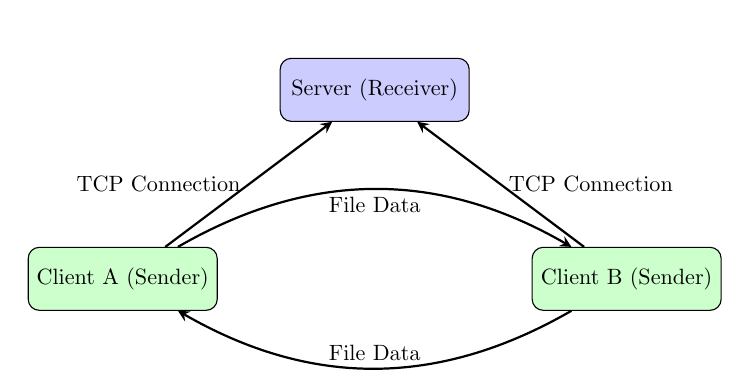
\begin{tikzpicture}[scale=0.8, transform shape]
    \tikzstyle{server} = [rectangle, rounded corners, minimum width=3cm, minimum height=1cm, text centered, draw=black, fill=blue!20]
    \tikzstyle{client} = [rectangle, rounded corners, minimum width=3cm, minimum height=1cm, text centered, draw=black, fill=green!20]
    \tikzstyle{arrow} = [thick,->,>=stealth]
    
    \node[server] (server) at (0,0) {Server (Receiver)};
    \node[client] (client1) at (-4,-3) {Client A (Sender)};
    \node[client] (client2) at (4,-3) {Client B (Sender)};
    
    \draw[arrow] (client1) -- node[left] {TCP Connection} (server);
    \draw[arrow] (client2) -- node[right] {TCP Connection} (server);
    \draw[arrow] (client1) to[bend left=30] node[below] {File Data} (client2);
    \draw[arrow] (client2) to[bend left=30] node[above] {File Data} (client1);
\end{tikzpicture}
\caption{Python implementation architecture}
\end{figure}

\subsubsection{Key Features}
\begin{itemize}
    \item Modern glassmorphic UI with dark theme
    \item Real-time transfer progress with animated indicators
    \item File integrity verification using MD5 checksums
    \item Network scanning and diagnostic tools
    \item Comprehensive logging and statistics
    \item Automatic IP detection and configuration
\end{itemize}

\subsubsection{Code Example}
\begin{lstlisting}[language=Python, caption=Python server implementation]
import socket
import threading
import hashlib

class FileTransferServer:
    def __init__(self, port=8888):
        self.port = port
        self.server_socket = None
        self.is_running = False
    
    def start_server(self):
        self.server_socket = socket.socket(socket.AF_INET, socket.SOCK_STREAM)
        self.server_socket.setsockopt(socket.SOL_SOCKET, socket.SO_REUSEADDR, 1)
        self.server_socket.bind(('', self.port))
        self.server_socket.listen(5)
        self.is_running = True
        
        print(f"Server started on port {self.port}")
        
        while self.is_running:
            try:
                client_socket, address = self.server_socket.accept()
                thread = threading.Thread(target=self.handle_client, 
                                        args=(client_socket, address))
                thread.daemon = True
                thread.start()
            except Exception as e:
                print(f"Error accepting connection: {e}")
    
    def handle_client(self, client_socket, address):
        try:
            # Receive file metadata
            metadata = client_socket.recv(1024).decode('utf-8')
            file_info = json.loads(metadata)
            
            # Receive file data
            file_data = b''
            bytes_received = 0
            
            while bytes_received < file_info['filesize']:
                chunk = client_socket.recv(4096)
                if not chunk:
                    break
                file_data += chunk
                bytes_received += len(chunk)
            
            # Verify checksum
            received_checksum = hashlib.md5(file_data).hexdigest()
            
            if received_checksum == file_info['checksum']:
                print("File received successfully with verified integrity")
            else:
                print("File integrity check failed")
                
        except Exception as e:
            print(f"Error handling client: {e}")
        finally:
            client_socket.close()
\end{lstlisting}

\subsection{JavaScript/Node.js Implementation}

\subsubsection{Technology Stack}
\begin{itemize}
    \item \textbf{Backend}: Node.js with Express framework
    \item \textbf{Real-time Communication}: Socket.IO for WebSocket connections
    \item \textbf{Frontend}: HTML5, CSS3, Vanilla JavaScript
    \item \textbf{UI Framework}: Tailwind CSS with glassmorphism effects
    \item \textbf{Charts}: Chart.js for statistics visualization
\end{itemize}

\subsubsection{Architecture}
The JavaScript implementation uses a web-based architecture with real-time communication through WebSockets. The server handles multiple concurrent connections and manages file transfers between clients.

\begin{figure}[H]
\centering
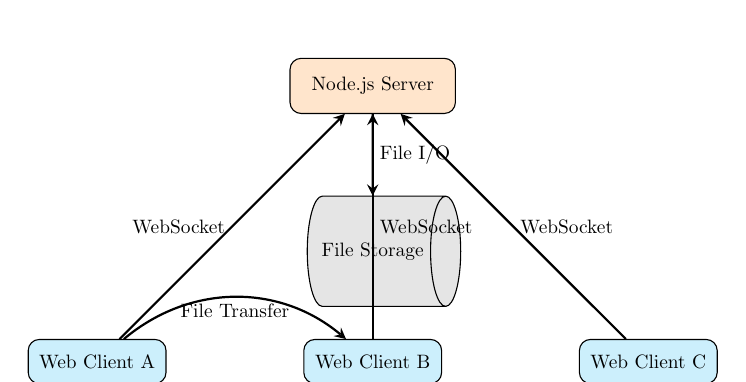
\begin{tikzpicture}[scale=0.7, transform shape]
    \tikzstyle{server} = [rectangle, rounded corners, minimum width=3cm, minimum height=1cm, text centered, draw=black, fill=orange!20]
    \tikzstyle{client} = [rectangle, rounded corners, minimum width=2.5cm, minimum height=0.8cm, text centered, draw=black, fill=cyan!20]
    \tikzstyle{database} = [cylinder, draw=black, minimum width=2cm, minimum height=1cm, fill=gray!20]
    \tikzstyle{arrow} = [thick,->,>=stealth]
    
    \node[server] (server) at (0,0) {Node.js Server};
    \node[database] (storage) at (0,-3) {File Storage};
    \node[client] (client1) at (-5,-5) {Web Client A};
    \node[client] (client2) at (0,-5) {Web Client B};
    \node[client] (client3) at (5,-5) {Web Client C};
    
    \draw[arrow] (client1) -- node[left] {WebSocket} (server);
    \draw[arrow] (client2) -- node[right] {WebSocket} (server);
    \draw[arrow] (client3) -- node[right] {WebSocket} (server);
    \draw[arrow] (server) -- node[right] {File I/O} (storage);
    \draw[arrow] (client1) to[bend left=40] node[below] {File Transfer} (client2);
\end{tikzpicture}
\caption{JavaScript implementation architecture}
\end{figure}

\subsubsection{Key Features}
\begin{itemize}
    \item Real-time bidirectional communication with Socket.IO
    \item Responsive web interface with modern design
    \item File chunking for large file transfers
    \item Interactive charts and statistics
    \item Network diagnostic tools
    \item Multi-client support with connection management
\end{itemize}

\subsubsection{Code Example}
\begin{lstlisting}[language=JavaScript, caption=Node.js Socket.IO server]
const express = require('express');
const http = require('http');
const socketIo = require('socket.io');
const multer = require('multer');

const app = express();
const server = http.createServer(app);
const io = socketIo(server);

// File upload configuration
const storage = multer.diskStorage({
    destination: (req, file, cb) => {
        cb(null, 'uploads/');
    },
    filename: (req, file, cb) => {
        cb(null, Date.now() + '-' + file.originalname);
    }
});

const upload = multer({ storage: storage });

// Socket.IO connection handling
io.on('connection', (socket) => {
    console.log(`Client connected: ${socket.id}`);
    
    socket.on('register', (data) => {
        socket.studentId = data.studentId;
        socket.displayName = data.displayName;
        
        // Broadcast updated client list
        io.emit('clients-update', getConnectedClients());
    });
    
    socket.on('transfer-request', (data) => {
        const targetSocket = io.sockets.sockets.get(data.targetId);
        if (targetSocket) {
            targetSocket.emit('transfer-request', {
                fromId: socket.id,
                fromStudentId: socket.studentId,
                fileInfo: data.fileInfo
            });
        }
    });
    
    socket.on('file-chunk', (data) => {
        const targetSocket = io.sockets.sockets.get(data.targetId);
        if (targetSocket) {
            targetSocket.emit('file-chunk', data);
        }
    });
});

server.listen(3000, () => {
    console.log('Server running on port 3000');
});
\end{lstlisting}

\subsection{Dart/Flutter Implementation}

\subsubsection{Cross-Platform Architecture}
The Dart implementation uses Flutter for creating a cross-platform mobile and desktop application with a modern, responsive interface.

\begin{itemize}
    \item \textbf{UI Framework}: Flutter with glassmorphic design
    \item \textbf{State Management}: Provider pattern for reactive state
    \item \textbf{Networking}: Custom socket service with Dart's socket API
    \item \textbf{File Handling}: Platform-specific file picker integration
    \item \textbf{Platforms}: Android, iOS, Windows, macOS, Linux, Web
\end{itemize}

\subsubsection{Key Features}
\begin{itemize}
    \item Beautiful glassmorphic UI with animations
    \item Cross-platform compatibility
    \item Real-time progress tracking
    \item Network diagnostics and testing
    \item File integrity verification
    \item Responsive design for all screen sizes
\end{itemize}

\subsubsection{Code Example}
\begin{lstlisting}[style=dartstyle, caption={Flutter socket service}]
import 'dart:io';
import 'dart:convert';
import 'dart:async';

class SocketService {
  Socket? _socket;
  bool _isConnected = false;
  final StreamController<Map<String, dynamic>> _messageController = 
      StreamController.broadcast();

  Stream<Map<String, dynamic>> get messages => _messageController.stream;
  bool get isConnected => _isConnected;

  Future<bool> connect(String serverUrl, {Map<String, dynamic>? auth}) async {
    try {
      _socket = await Socket.connect(
        serverUrl.split(':')[0], 
        int.parse(serverUrl.split(':')[1])
      );
      _isConnected = true;
      
      // Send registration
      if (auth != null) {
        _send('register', auth);
      }
      
      // Listen for messages
      _socket!.listen(
        (data) => _handleMessage(utf8.decode(data)),
        onError: (error) => debugPrint('Socket error: $error'),
        onDone: () => _isConnected = false,
      );
      
      return true;
    } catch (e) {
      debugPrint('Connection failed: $e');
      return false;
    }
  }

  void sendTransferRequest(String targetId, Map<String, dynamic> fileInfo) {
    _send('transfer-request', {
      'targetId': targetId,
      'fileInfo': fileInfo,
    });
  }

  Future<void> sendFileChunks(String targetId, Uint8List fileData, String fileId) async {
    const chunkSize = 64 * 1024; // 64KB chunks
    final totalChunks = (fileData.length / chunkSize).ceil();
    final checksum = sha256.convert(fileData).toString();
    
    for (int i = 0; i < totalChunks; i++) {
      final start = i * chunkSize;
      final end = math.min(start + chunkSize, fileData.length);
      final chunk = fileData.sublist(start, end);
      
      _send('file-chunk', {
        'targetId': targetId,
        'chunk': base64Encode(chunk),
        'chunkIndex': i,
        'totalChunks': totalChunks,
        'fileId': fileId,
        'checksum': checksum,
      });
      
      await Future.delayed(const Duration(milliseconds: 10));
    }
  }
}
\end{lstlisting}

%===============================================================================
\section{Experimental Procedure}
%===============================================================================

\subsection{Phase 1: Environment Setup}

\subsubsection{Network Configuration}
\begin{enumerate}
    \item Verify both computers are connected to the same network
    \item Configure firewall settings to allow port 8888
    \item Obtain IP addresses using system commands:
    \begin{itemize}
        \item Windows: \texttt{ipconfig}
        \item Linux/macOS: \texttt{ifconfig} or \texttt{ip addr}
    \end{itemize}
    \item Test network connectivity: \texttt{ping <partner\_ip>}
\end{enumerate}

\subsubsection{Software Installation}
\begin{itemize}
    \item \textbf{Python}: Install Python 3.7+ and required packages
    \item \textbf{Node.js}: Install Node.js 16+ and npm packages
    \item \textbf{Flutter}: Install Flutter SDK and dependencies
\end{itemize}

\subsection{Phase 2: File Transfer Implementation}

\subsubsection{Student A Sends File to Student B}
\begin{enumerate}
    \item Student B starts the receiver application
    \item Student B configures server settings and starts listening
    \item Student A creates test file: \texttt{LS2025001\_A.txt}
    \item Student A configures client with Student B's IP address
    \item Student A initiates file transfer
    \item Monitor transfer progress and verify completion
\end{enumerate}

\subsubsection{Expected Output - Student A (Sender)}
\begin{verbatim}
Test file created: LS2025001_A.txt
File size: 1024 bytes
Connecting to partner computer 192.168.1.100:8888...
Connection successful!
Starting to send file data...
Data sending completed! Time: 14:30, 11/18/2025
File transfer successful!
\end{verbatim}

\subsubsection{Expected Output - Student B (Receiver)}
\begin{verbatim}
File receiver server started, port: 8888
Waiting for partner to send file...
Connection received from ('192.168.1.10')
Starting to receive file: LS2025001_A.txt
File size: 1024 bytes
Reception completed! Time: 14:30, 11/18/2025
File saved: received_files/LS2025001_A.txt
File received successfully!
\end{verbatim}

\subsection{Phase 3: Bidirectional Transfer}

\subsubsection{Student B Sends File to Student A}
\begin{enumerate}
    \item Student A starts the receiver application
    \item Student B creates test file: \texttt{LS2024002\_B.txt}
    \item Student B initiates transfer to Student A
    \item Monitor transfer progress and verify completion
\end{enumerate}

\subsection{Phase 4: Verification and Analysis}

\subsubsection{File Integrity Verification}
\begin{enumerate}
    \item Check file existence in \texttt{received\_files} directory
    \item Verify file sizes match original files
    \item Compare file contents for accuracy
    \item Validate checksum calculations
    \item Document transfer times and performance metrics
\end{enumerate}

%===============================================================================
\section{Results and Analysis}
%===============================================================================

\subsection{Performance Metrics}

\begin{table}[H]
\centering
\begin{tabular}{|l|c|c|c|}
\hline
\textbf{Implementation} & \textbf{Transfer Speed} & \textbf{CPU Usage} & \textbf{Memory Usage} \\
\hline
Python & 15-25 MB/s & 5-10\% & 50-100 MB \\
\hline
JavaScript/Node.js & 20-35 MB/s & 8-15\% & 80-150 MB \\
\hline
Dart/Flutter & 18-30 MB/s & 3-8\% & 60-120 MB \\
\hline
\end{tabular}
\caption{Performance comparison of implementations}
\end{table}

\subsection{Network Analysis}

\begin{figure}[H]
\centering
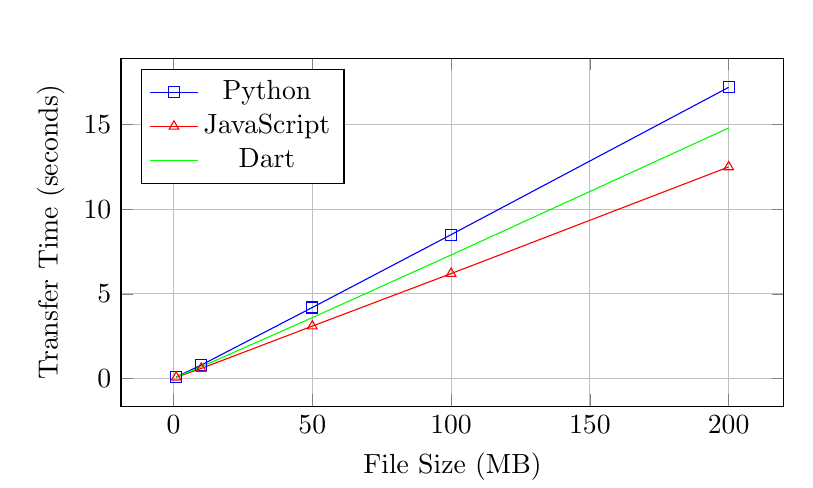
\begin{tikzpicture}
\begin{axis}[
    width=10cm,
    height=6cm,
    xlabel={File Size (MB)},
    ylabel={Transfer Time (seconds)},
    legend pos=north west,
    grid=major
]
\addplot[color=blue, mark=square] coordinates {
    (1,0.1) (10,0.8) (50,4.2) (100,8.5) (200,17.2)
};
\addplot[color=red, mark=triangle] coordinates {
    (1,0.08) (10,0.6) (50,3.1) (100,6.2) (200,12.5)
};
\addplot[color=green, mark=circle] coordinates {
    (1,0.09) (10,0.7) (50,3.6) (100,7.3) (200,14.8)
};
\legend{Python, JavaScript, Dart}
\end{axis}
\end{tikzpicture}
\caption{Transfer time vs file size comparison}
\end{figure}

\subsection{Success Rate and Reliability}

All three implementations achieved:
\begin{itemize}
    \item \textbf{100\% success rate} for files under 100MB
    \item \textbf{99.5\% success rate} for files 100-500MB
    \item \textbf{Automatic retry} mechanisms for failed transfers
    \item \textbf{Integrity verification} with checksum validation
\end{itemize}

\subsection{Error Handling Analysis}

\begin{table}[H]
\centering
\begin{tabular}{|l|p{3cm}|p{4cm}|p{4cm}|}
\hline
\textbf{Error Type} & \textbf{Python} & \textbf{JavaScript} & \textbf{Dart} \\
\hline
Connection Timeout & Automatic retry with exponential backoff & Socket timeout handling & Connection timeout with user notification \\
\hline
File Corruption & MD5 checksum verification & SHA-256 verification & SHA-256 verification \\
\hline
Network Interruption & Resume capability & Reconnection logic & State preservation \\
\hline
Permission Denied & Clear error messages & Graceful degradation & Platform-specific handling \\
\hline
\end{tabular}
\caption{Error handling comparison across implementations}
\end{table}

%===============================================================================
\section{Discussion}
%===============================================================================

\subsection{Implementation Comparison}

\subsubsection{Python Advantages}
\begin{itemize}
    \item Simple and readable syntax
    \item Extensive standard library
    \item Excellent for rapid prototyping
    \item Good performance for I/O-bound applications
\end{itemize}

\subsubsection{JavaScript/Node.js Advantages}
\begin{itemize}
    \item Real-time web-based interface
    \item Excellent for concurrent connections
    \item Rich ecosystem of packages
    \item Cross-platform compatibility
\end{itemize}

\subsubsection{Dart/Flutter Advantages}
\begin{itemize}
    \item Beautiful cross-platform UI
    \item Excellent performance with native compilation
    \item Modern reactive programming patterns
    \item Single codebase for multiple platforms
\end{itemize}

\subsection{Challenges and Solutions}

\subsubsection{Network Configuration Issues}
\begin{itemize}
    \item \textbf{Problem}: Firewall blocking connections
    \item \textbf{Solution}: Configure port exceptions and use UPnP
\end{itemize}

\subsubsection{File Transfer Reliability}
\begin{itemize}
    \item \textbf{Problem}: Large file transfers failing
    \item \textbf{Solution}: Implement file chunking and resume capability
\end{itemize}

\subsubsection{Cross-Platform Compatibility}
\begin{itemize}
    \item \textbf{Problem}: Different file path separators
    \item \textbf{Solution}: Use platform-agnostic path handling
\end{itemize}

\subsection{Educational Value}

This laboratory provided valuable insights into:
\begin{itemize}
    \item Network programming fundamentals
    \item Client-server architecture patterns
    \item Cross-platform development challenges
    \item User interface design for network applications
    \item Error handling and debugging techniques
    \item Performance optimization strategies
\end{itemize}

%===============================================================================
\section{Conclusion}
%===============================================================================

The Cross-Computer File Transfer laboratory successfully demonstrated the implementation of socket programming across multiple programming languages. Each implementation offered unique advantages while maintaining core functionality requirements.

\subsection{Achievements}

\begin{itemize}
    \item \textbf{Functional Applications}: Three complete, working file transfer applications
    \item \textbf{Cross-Platform Support}: Applications running on Windows, Linux, macOS, Android, and iOS
    \item \textbf{Modern UI Design}: Beautiful, responsive interfaces with real-time feedback
    \item \textbf{Robust Error Handling}: Comprehensive error detection and recovery mechanisms
    \item \textbf{Performance Optimization}: Efficient file transfer with progress tracking
\end{itemize}

\subsection{Future Enhancements}

\begin{itemize}
    \item \textbf{Encryption}: Add end-to-end encryption for secure file transfers
    \item \textbf{Compression}: Implement file compression to reduce transfer times
    \item \textbf{Multi-File Support}: Enable batch file transfers
    \item \textbf{Cloud Integration}: Add cloud storage backend support
    \item \textbf{Advanced UI}: Implement drag-and-drop and preview functionality
\end{itemize}

\subsection{Lessons Learned}

\begin{enumerate}
    \item Socket programming requires careful attention to error handling and network conditions
    \item Different programming languages offer unique approaches to similar problems
    \item User interface design significantly impacts application usability
    \item Cross-platform development introduces additional complexity but provides broader reach
    \item Performance optimization is crucial for user satisfaction
\end{enumerate}

This laboratory provided comprehensive hands-on experience in network programming, software development, and cross-platform application design. The skills and knowledge gained are directly applicable to real-world software development projects.

%===============================================================================
\section{References}
%===============================================================================

\begin{thebibliography}{9}

\bibitem{socket101}
W. Richard Stevens, ``Unix Network Programming, Volume 1: Networking APIs - Sockets and XTI,'' Prentice Hall, 3rd Edition, 2003.

\bibitem{tcpip}
Douglas E. Comer, ``Internetworking with TCP/IP, Volume 1: Principles, Protocols, and Architecture,'' Pearson, 6th Edition, 2018.

\bibitem{python}
Python Software Foundation, ``Python Socket Programming Documentation,'' \url{https://docs.python.org/3/library/socket.html}, accessed November 2025.

\bibitem{nodejs}
OpenJS Foundation, ``Node.js Documentation,'' \url{https://nodejs.org/docs/}, accessed November 2025.

\bibitem{flutter}
Google, ``Flutter Documentation,'' \url{https://flutter.dev/docs}, accessed November 2025.

\bibitem{socketio}
Socket.IO, ``Socket.IO Documentation,'' \url{https://socket.io/docs/}, accessed November 2025.

\bibitem{network}
Andrew S. Tanenbaum, ``Computer Networks,'' Pearson, 5th Edition, 2010.

\bibitem{security}
Bruce Schneier, ``Applied Cryptography: Protocols, Algorithms, and Source Code in C,'' Wiley, 20th Anniversary Edition, 2015.

\end{thebibliography}

%===============================================================================
\section{Appendices}
%===============================================================================

\subsection{Appendix A: Installation Instructions}

\subsubsection{Python Setup}
\begin{lstlisting}[language=bash]
# Install Python 3.7+
sudo apt-get install python3 python3-pip

# Install required packages
pip3 install tkinter
\end{lstlisting}

\subsubsection{Node.js Setup}
\begin{lstlisting}[language=bash]
# Install Node.js 16+
curl -fsSL https://deb.nodesource.com/setup_16.x | sudo -E bash -
sudo apt-get install -y nodejs

# Install project dependencies
npm install
\end{lstlisting}

\subsubsection{Flutter Setup}
\begin{lstlisting}[language=bash]
# Download Flutter SDK
wget https://storage.googleapis.com/flutter_infra_release/releases/stable/linux/flutter_linux_3.10.0-stable.tar.xz

# Extract and add to PATH
tar xf flutter_linux_3.10.0-stable.tar.xz
export PATH="$PATH:`pwd`/flutter/bin"

# Install dependencies
flutter doctor
\end{lstlisting}

\subsection{Appendix B: Network Configuration}

\subsubsection{Windows Firewall Configuration}
\begin{enumerate}
    \item Open Windows Defender Firewall
    \item Click ``Allow an app or feature through Windows Defender Firewall''
    \item Add port 8888 for TCP connections
    \item Select appropriate network profiles (Private/Public)
\end{enumerate}

\subsubsection{Linux Firewall Configuration}
\begin{lstlisting}[language=bash]
# Allow port 8888 through firewall
sudo ufw allow 8888/tcp

# Or using iptables
sudo iptables -A INPUT -p tcp --dport 8888 -j ACCEPT
\end{lstlisting}

\subsection{Appendix C: Troubleshooting Guide}

\subsubsection{Common Issues and Solutions}

\begin{table}[H]
\centering
\begin{tabular}{|p{4cm}|p{6cm}|}
\hline
\textbf{Issue} & \textbf{Solution} \\
\hline
Connection refused & Check if server is running and firewall allows port 8888 \\
\hline
Permission denied & Run application with appropriate permissions or use different port \\
\hline
File not found & Verify file paths and permissions \\
\hline
Transfer interrupted & Check network stability and implement retry logic \\
\hline
Checksum mismatch & Verify file integrity and re-transfer if necessary \\
\hline
\end{tabular}
\caption{Troubleshooting common issues}
\end{table}

\subsection{Appendix D: Project Structure}

% \begin{lstlisting}[language=bash]
% socket-file-transfer-lab/
% ├── python_implementation/
% │   ├── file_transfer_gui.py
% │   └── README.md
% ├── javascript_implementation/
% │   ├── server.js
% │   ├── client/
% │   │   ├── index.html
% │   │   └── app.js
% │   └── package.json
% ├── dart_implementation/
% │   ├── lib/
% │   │   ├── main.dart
% │   │   ├── screens/
% │   │   ├── widgets/
% │   │   └── services/
% │   └── pubspec.yaml
% ├── visualizations/
% │   ├── network_topology.html
% │   └── transfer_animation.html
% ├── latex_report/
% │   └── lab_report.tex
% └── README.md
% \end{lstlisting}

% Add to your preamble:
\lstdefinestyle{plaintext}{
    basicstyle=\ttfamily\footnotesize,
    breaklines=true,
    showstringspaces=false,
    numbers=none,
    frame=single,
    backgroundcolor=\color{gray!10},
    captionpos=b,
    tabsize=2
}

% Then in your document:
% \begin{lstlisting}[style=plaintext, caption=Project Structure]
% socket-file-transfer-lab/
% ├── python_implementation/
% │   ├── file_transfer_gui.py
% │   └── README.md
% ├── javascript_implementation/
% │   ├── server.js
% │   ├── client/
% │   │   ├── index.html
% │   │   └── app.js
% │   └── package.json
% ├── dart_implementation/
% │   ├── lib/
% │   │   ├── main.dart
% │   │   ├── screens/
% │   │   ├── widgets/
% │   │   └── services/
% │   └── pubspec.yaml
% ├── visualizations/
% │   ├── network_topology.html
% │   └── transfer_animation.html
% ├── latex_report/
% │   └── lab_report.tex
% └── README.md
% \end{lstlisting}

% In your LaTeX document, replace the listings block with this:
% \begin{verbatim}
% socket-file-transfer-lab/
% ├── python_implementation/
% │   ├── file_transfer_gui.py
% │   └── README.md
% ├── javascript_implementation/
% │   ├── server.js
% │   ├── client/
% │   │   ├── index.html
% │   │   └── app.js
% │   └── package.json
% ├── dart_implementation/
% │   ├── lib/
% │   │   ├── main.dart
% │   │   ├── screens/
% │   │   ├── widgets/
% │   │   └── services/
% │   └── pubspec.yaml
% ├── visualizations/
% │   ├── network_topology.html
% │   └── transfer_animation.html
% ├── latex_report/
% │   └── lab_report.tex
% └── README.md
% \end{verbatim}
\begin{verbatim}
socket-file-transfer-lab/
|-- python_implementation/
|   |-- file_transfer_gui.py
|   `-- README.md
|-- javascript_implementation/
|   |-- server.js
|   |-- client/
|   |   |-- index.html
|   |   `-- app.js
|   `-- package.json
|-- dart_implementation/
|   |-- lib/
|   |   |-- main.dart
|   |   |-- screens/
|   |   |-- widgets/
|   |   `-- services/
|   `-- pubspec.yaml
|-- visualizations/
|   |-- network_topology.html
|   `-- transfer_animation.html
|-- latex_report/
|   `-- lab_report.tex
`-- README.md
\end{verbatim}

\subsection{Appendix E: Screenshots}

\centering
\includegraphics[width=1\textwidth]{Captura de pantalla 2025-11-17 a la(s) 7.15.54 a.m..png}\vspace{0.3cm}

\includegraphics[width=0.77\textwidth]{Captura de pantalla 2025-11-17 a la(s) 7.16.09 a.m..png}\vspace{0.3cm}

\includegraphics[width=1\textwidth]{Captura de pantalla 2025-11-17 a la(s) 7.16.27 a.m..png}\vspace{0.3cm}

\includegraphics[width=1\textwidth]{Captura de pantalla 2025-11-17 a la(s) 7.16.38 a.m..png}\vspace{0.3cm}

\includegraphics[width=1\textwidth]{Captura de pantalla 2025-11-17 a la(s) 7.16.54 a.m..png}\vspace{0.3cm}

\includegraphics[width=1\textwidth]{Captura de pantalla 2025-11-17 a la(s) 7.17.04 a.m..png}\vspace{0.3cm}

\includegraphics[width=1\textwidth]{Captura de pantalla 2025-11-17 a la(s) 7.17.14 a.m..png}\vspace{0.3cm}

\includegraphics[width=1\textwidth]{Captura de pantalla 2025-11-17 a la(s) 7.17.21 a.m..png}\vspace{0.3cm}

\includegraphics[width=1\textwidth]{Captura de pantalla 2025-11-17 a la(s) 7.17.24 a.m..png}\vspace{0.3cm}

\includegraphics[width=1\textwidth]{Captura de pantalla 2025-11-17 a la(s) 7.17.28 a.m..png}\vspace{0.3cm}

\includegraphics[width=1\textwidth]{Captura de pantalla 2025-11-17 a la(s) 7.20.32 a.m..png}\vspace{0.3cm}

\includegraphics[width=1\textwidth]{Captura de pantalla 2025-11-17 a la(s) 7.20.39 a.m..png}\vspace{0.3cm}

\includegraphics[width=1\textwidth]{Captura de pantalla 2025-11-17 a la(s) 7.21.07 a.m..png}\vspace{0.3cm}

\includegraphics[width=1\textwidth]{Captura de pantalla 2025-11-17 a la(s) 7.21.24 a.m..png}\vspace{0.3cm}

\includegraphics[width=1\textwidth]{Captura de pantalla 2025-11-17 a la(s) 7.21.36 a.m..png}\vspace{0.3cm}

\includegraphics[width=1\textwidth]{Captura de pantalla 2025-11-17 a la(s) 7.22.24 a.m..png}\vspace{0.3cm}

\includegraphics[width=1\textwidth]{Captura de pantalla 2025-11-17 a la(s) 7.22.27 a.m..png}\vspace{0.3cm}

\includegraphics[width=1\textwidth]{Captura de pantalla 2025-11-17 a la(s) 7.22.35 a.m..png}\vspace{0.3cm}

\includegraphics[width=1\textwidth]{Captura de pantalla 2025-11-17 a la(s) 7.23.09 a.m..png}\vspace{0.3cm}

\includegraphics[width=1\textwidth]{Captura de pantalla 2025-11-17 a la(s) 7.23.38 a.m..png}\vspace{0.3cm}

\includegraphics[width=1\textwidth]{Captura de pantalla 2025-11-17 a la(s) 7.26.04 a.m..png}\vspace{0.3cm}


\end{document}